\documentclass{beamer}
\usepackage[english]{babel}
\usepackage{amsmath,amssymb,graphicx}

%%%%%%%%%% Start TeXmacs macros
\newcommand{\cdummy}{\cdot}
\newcommand{\nospace}{}
\newcommand{\tmmathbf}[1]{\ensuremath{\boldsymbol{#1}}}
\newcommand{\tmop}[1]{\ensuremath{\operatorname{#1}}}
\newcommand{\tmverbatim}[1]{\text{{\ttfamily{#1}}}}
%%%%%%%%%% End TeXmacs macros

\begin{document}

{\screens{\begin{frame}
  \
  
  \
  
  \
  
  \
  
  \
  
  \title{计算视觉与模式识别}
  
  \maketitle
\end{frame}}{\begin{frame}
  \frametitle{几何摄像机模型}
  
  \
  
  \resizebox{1\columnwidth}{!}{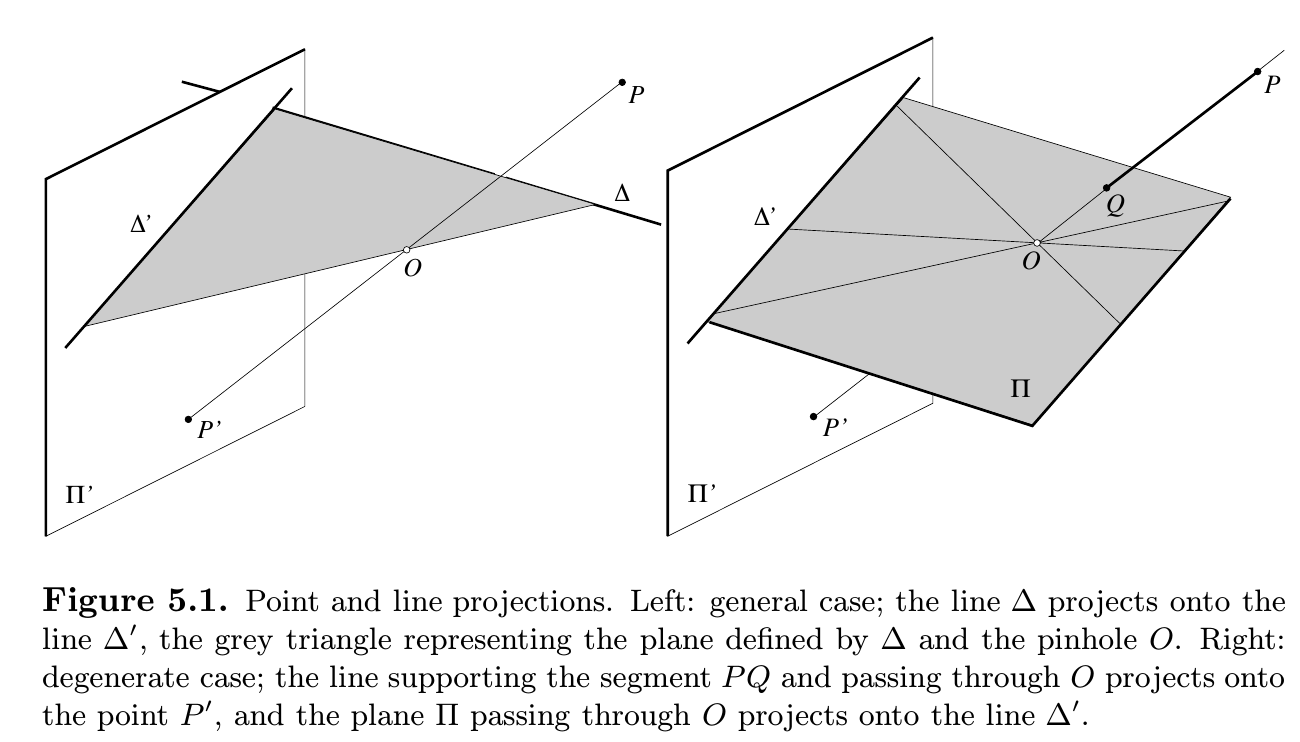
\includegraphics{img/point_line_projections.png}}
\end{frame}}{\begin{frame}
  \frametitle{坐标系}
  
  \resizebox{1\columnwidth}{!}{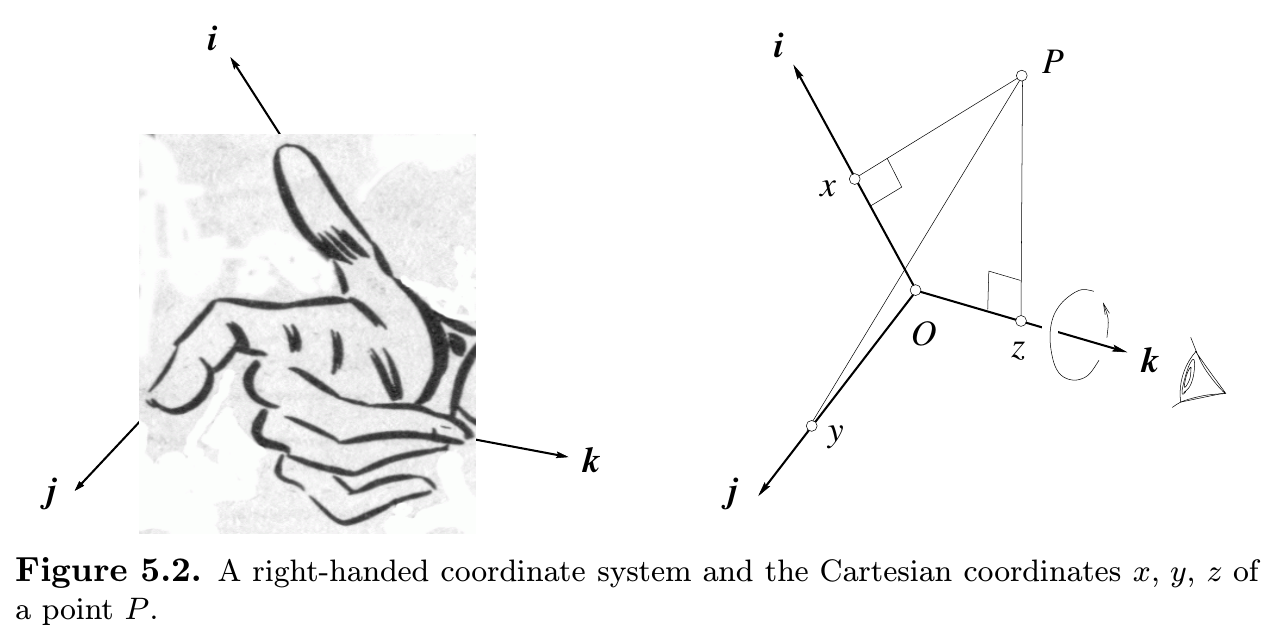
\includegraphics{img/coordinate_system.png}}
\end{frame}}{\begin{frame}
  \frametitle{}
  
  \resizebox{1\columnwidth}{!}{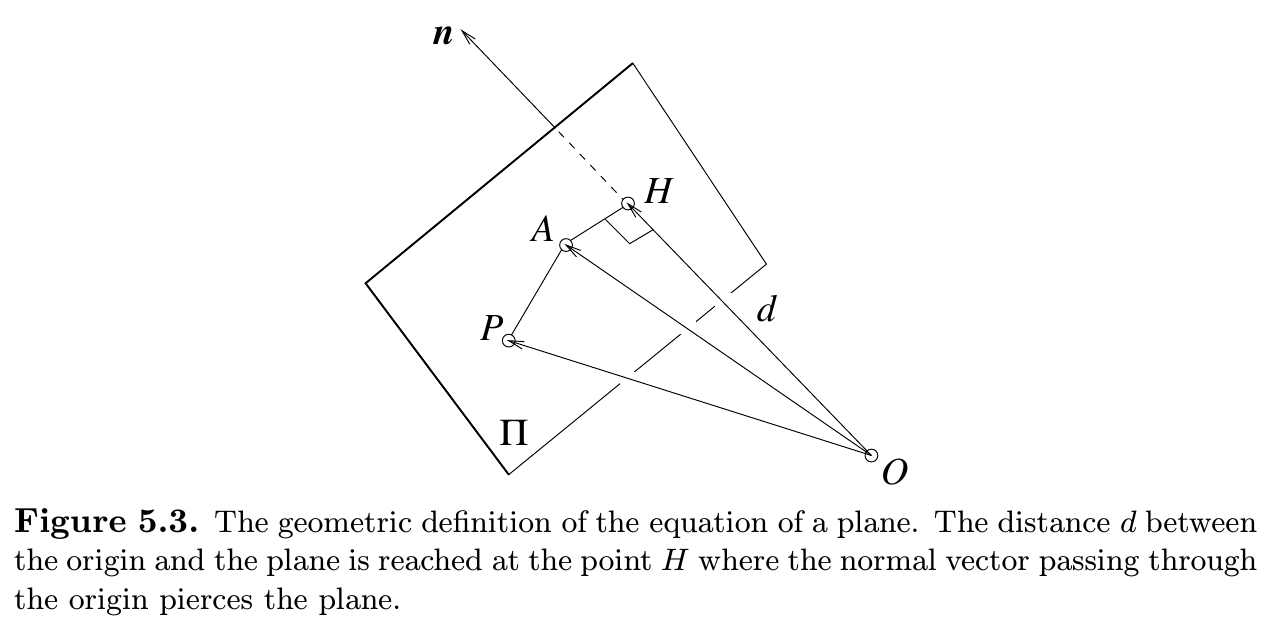
\includegraphics{img/plane_equation.png}}
\end{frame}}{\begin{frame}
  \frametitle{}
  \begin{eqnarray*}
    \overrightarrow{\tmop{OP}} & = & x\tmmathbf{i}+ y\tmmathbf{j}+
    z\tmmathbf{k}
  \end{eqnarray*}
  where
  \begin{eqnarray*}
    x & = & \overrightarrow{\tmop{OP}} \cdummy \tmmathbf{i}\\
    y & = & \overrightarrow{\tmop{OP}} \cdummy \tmmathbf{j}\\
    z & = & \overrightarrow{\tmop{OP}} \cdummy \tmmathbf{k}
  \end{eqnarray*}
  and
  \begin{eqnarray*}
    \tmmathbf{P} & = & \left(\begin{array}{c}
      x\\
      y\\
      z
    \end{array}\right) \in \mathbb{R}^3
  \end{eqnarray*}
\end{frame}}{\begin{frame}
  \frametitle{齐次坐标}
  \begin{eqnarray*}
    \left(\begin{array}{cccc}
      a & b & c & - d
    \end{array}\right) \left(\begin{array}{c}
      x\\
      y\\
      z\\
      1
    \end{array}\right) & = & 0\\
    \tmmathbf{\Pi} \cdummy \tmmathbf{P} & = & 0\\
    \tmmathbf{\Pi} & \equiv & \left(\begin{array}{c}
      a\\
      b\\
      c\\
      - d
    \end{array}\right)\\
    \tmmathbf{P} & \equiv & \left(\begin{array}{c}
      x\\
      y\\
      z\\
      1
    \end{array}\right)
  \end{eqnarray*}
  
\end{frame}}{\begin{frame}
  \frametitle{坐标变换------平移}
  
  \resizebox{1\columnwidth}{!}{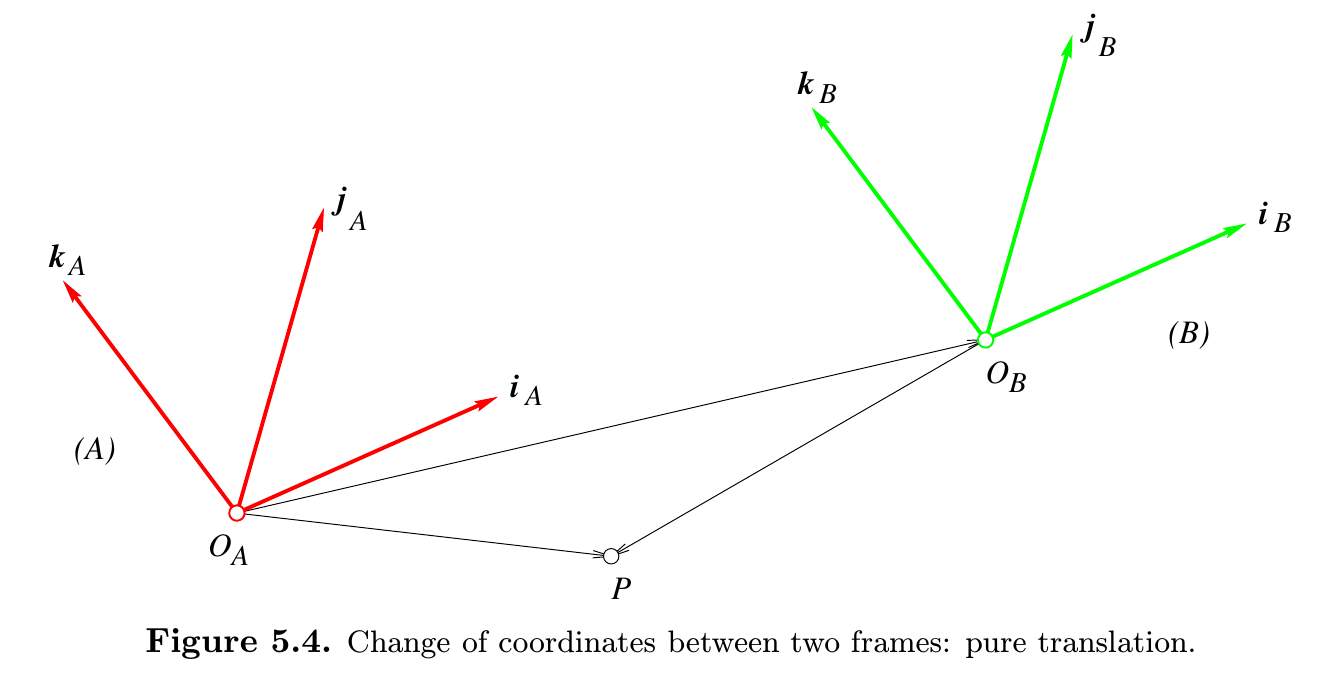
\includegraphics{img/pure_translation.png}}
\end{frame}}{\begin{frame}
  \frametitle{}
  \begin{eqnarray*}
    \overrightarrow{\tmop{OP}} & = & x\tmmathbf{i}+ y\tmmathbf{j}+
    z\tmmathbf{k}\\
    {}^F P & = & {}^F \overrightarrow{\tmop{OP}}\\
    & = & \left(\begin{array}{c}
      x\\
      y\\
      z
    \end{array}\right)\\
    {}^B P & = & {}^A P + {}^B O_A
  \end{eqnarray*}
\end{frame}}{\begin{frame}
  \frametitle{坐标变换------旋转}
  
  \resizebox{1\columnwidth}{!}{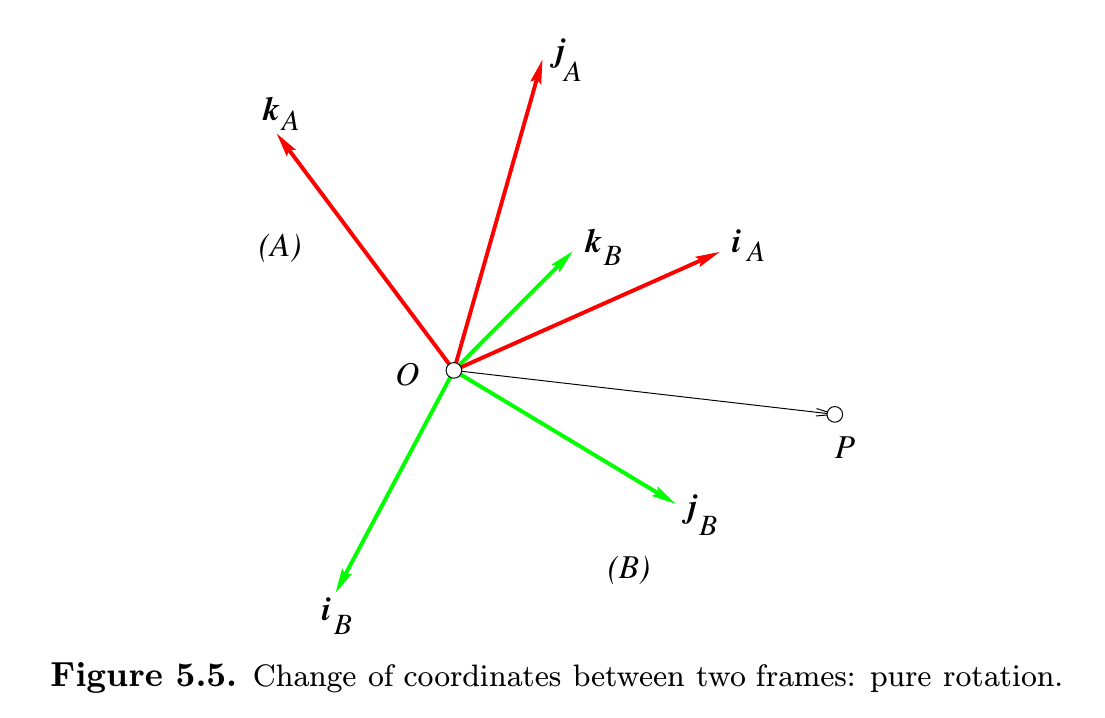
\includegraphics{img/pure_rotation.png}}
\end{frame}}{\begin{frame}
  
  \begin{eqnarray*}
    \overrightarrow{\tmop{OP}} & = & \left(\begin{array}{ccc}
      \tmmathbf{i}_A & \tmmathbf{j}_A & \tmmathbf{k}_A
    \end{array}\right) \left(\begin{array}{c}
      A_x\\
      A_y\\
      A_z
    \end{array}\right)\\
    & = & \left(\begin{array}{ccc}
      \tmmathbf{i}_B & \tmmathbf{j}_B & \tmmathbf{k}_B
    \end{array}\right) \left(\begin{array}{c}
      B_x\\
      B_y\\
      B_z
    \end{array}\right)
  \end{eqnarray*}
  \begin{eqnarray*}
    {}^B P & = & {}^B {}_A \mathcal{R} {}^A P
  \end{eqnarray*}
  \begin{eqnarray*}
    {}^B {}_A \mathcal{R} & = & \left(\begin{array}{ccc}
      \tmmathbf{i}_B & \tmmathbf{j}_B & \tmmathbf{k}_B
    \end{array}\right)^{^T} \left(\begin{array}{ccc}
      \tmmathbf{i}_A & \tmmathbf{j}_A & \tmmathbf{k}_A
    \end{array}\right)\\
    & = & \left(\begin{array}{ccc}
      \tmmathbf{i}_B \cdummy \tmmathbf{i}_A & \tmmathbf{i}_B \cdummy
      \tmmathbf{j}_A & \tmmathbf{i}_B \cdummy \tmmathbf{k}_A\\
      \tmmathbf{j}_B \cdummy \tmmathbf{i}_A & \tmmathbf{j}_B \cdummy
      \tmmathbf{j}_A & \tmmathbf{j}_B \cdummy \tmmathbf{k}_A\\
      \tmmathbf{k}_B \cdummy \tmmathbf{i}_A & \tmmathbf{k}_B \cdummy
      \tmmathbf{j}_A & \tmmathbf{k}_B \cdummy \tmmathbf{k}_A
    \end{array}\right)
  \end{eqnarray*}
  
\end{frame}}{\begin{frame}
  \frametitle{}
  
  \resizebox{1\columnwidth}{!}{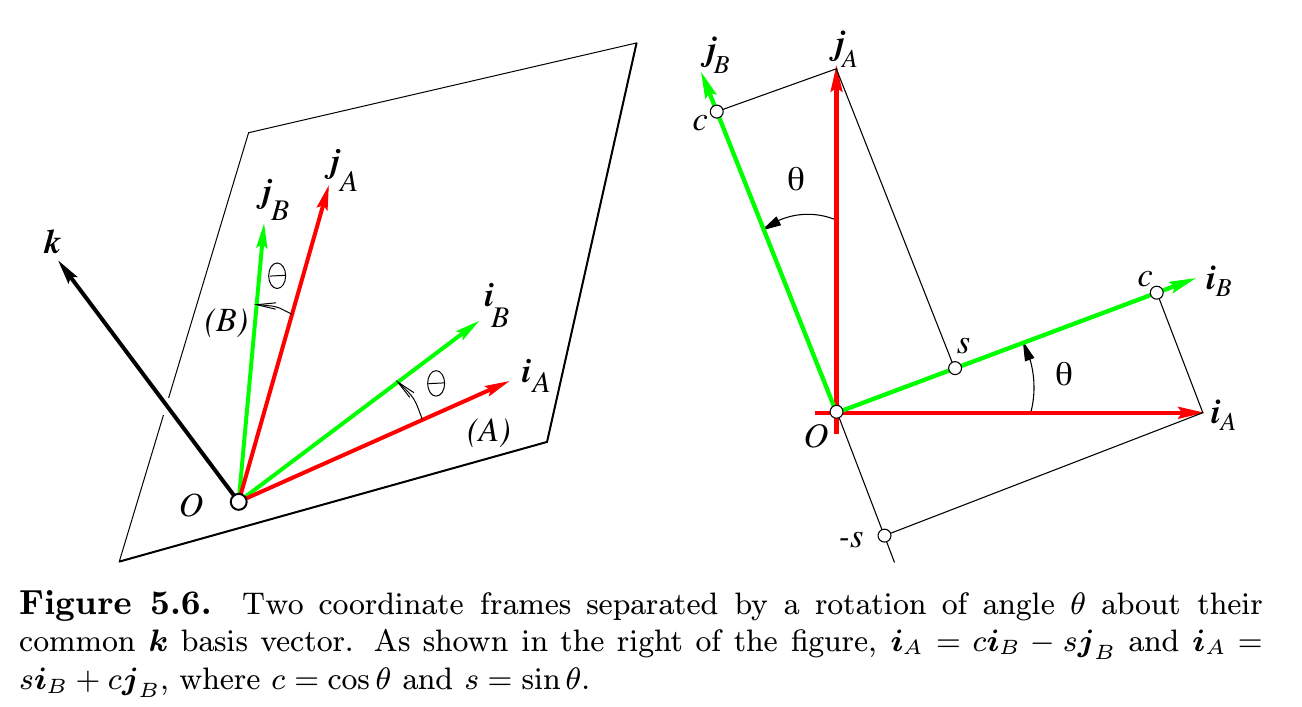
\includegraphics{img/rotation_of_theta.png}}
\end{frame}}{\begin{frame}
  \frametitle{}
  
  \
  
  \
  
  
  \begin{eqnarray*}
    {}^B {}_A \mathcal{R} & = & \left(\begin{array}{ccc}
      \cos \theta & \sin \theta & 0\\
      - \sin \theta & \cos \theta & 0\\
      0 & o & 1
    \end{array}\right)
  \end{eqnarray*}
\end{frame}}{\frametitle{坐标变换}

\resizebox{1\columnwidth}{!}{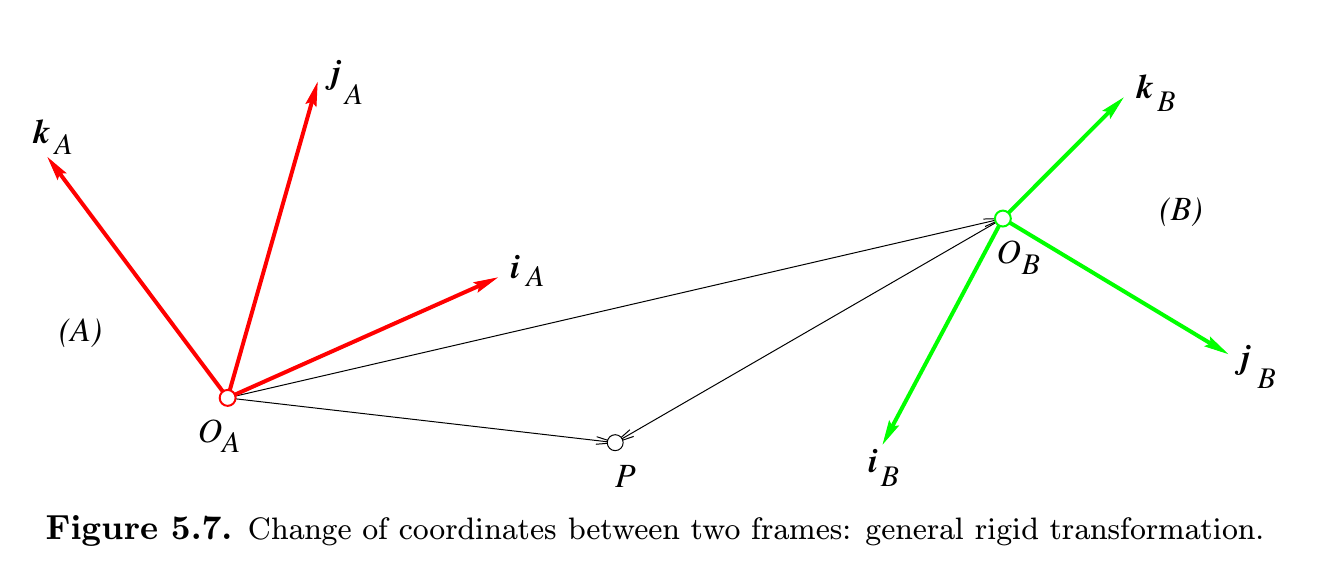
\includegraphics{img/rigid_transformation.png}}}{\begin{frame}
  \frametitle{}
  \begin{eqnarray*}
    \left(\begin{array}{c}
      {}^B P\\
      1
    \end{array}\right) & = & {}^B {}_A \mathcal{T} \left(\begin{array}{c}
      {}^A P\\
      1
    \end{array}\right)\\
    {}^B {}_A \mathcal{T} & \equiv & \left(\begin{array}{cc}
      {}^B {}_A \mathcal{R} & {}^B O_A\\
      \tmmathbf{0}^T & 1
    \end{array}\right)
  \end{eqnarray*}
\end{frame}}{\begin{frame}
  \frametitle{坐标旋转示例}
  
  \resizebox{1\columnwidth}{!}{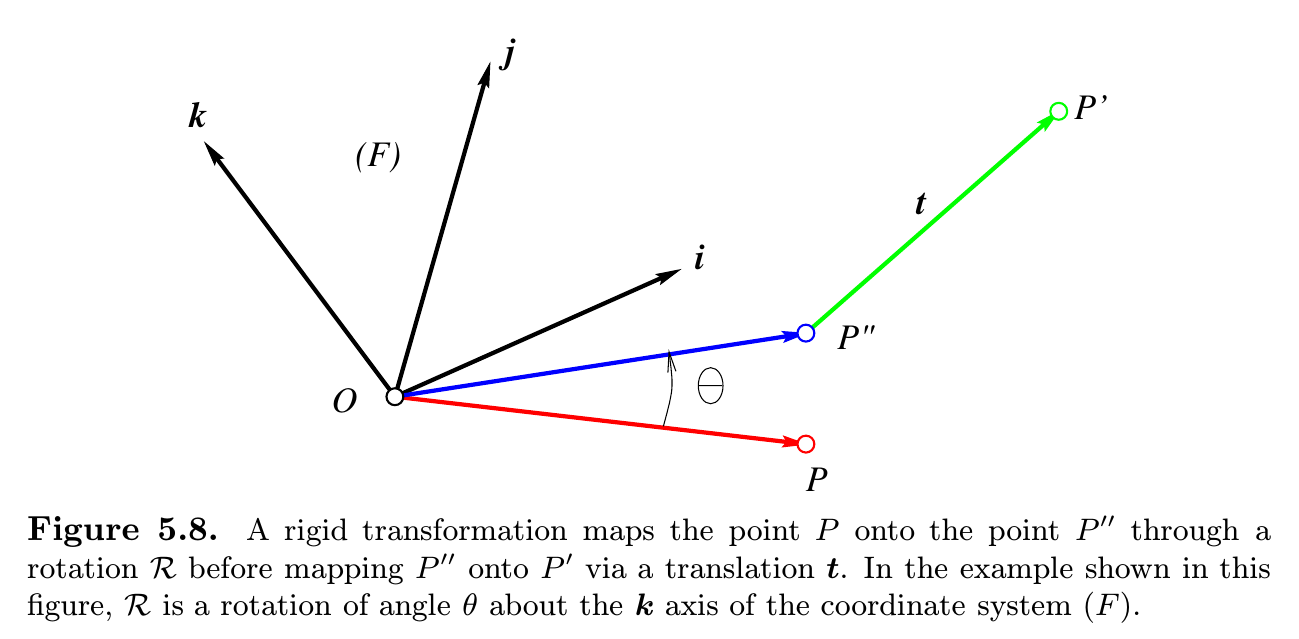
\includegraphics{img/mapping_p.png}}
\end{frame}}{\begin{frame}
  \frametitle{}
  
  \
  
  
  \begin{eqnarray*}
    {}^F P' & = & \mathcal{R}^F P
  \end{eqnarray*}
  where
  \begin{eqnarray*}
    \mathcal{R} & = & \left(\begin{array}{ccc}
      \cos \theta & - \sin \theta & 0\\
      \sin \theta & \cos \theta & 0\\
      0 & 0 & 1
    \end{array}\right)
  \end{eqnarray*}
\end{frame}}{\begin{frame}
  \frametitle{几何相机参数------内参数}
  
  \resizebox{1\columnwidth}{!}{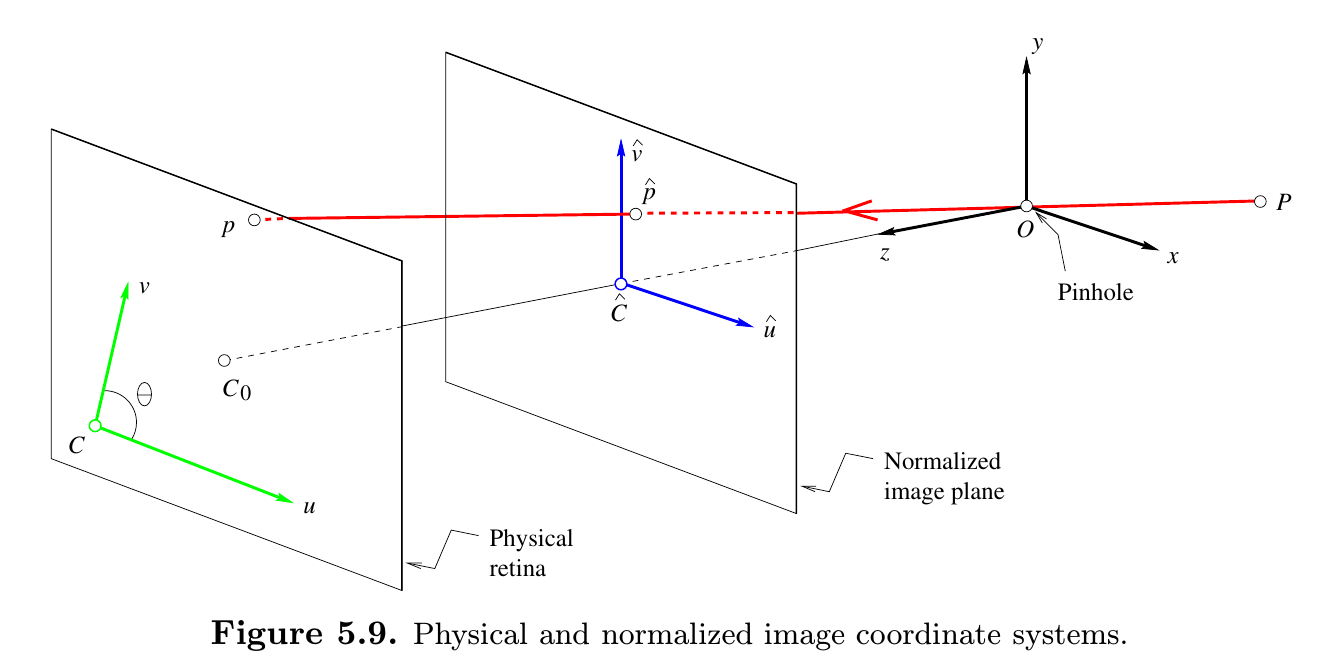
\includegraphics{img/physical_normal_image_coordinate_system.png}}
\end{frame}}{\begin{frame}
  \frametitle{}
  \begin{eqnarray*}
    \hat{\tmmathbf{P}} & = & \frac{1}{z} \left(\begin{array}{cc}
      \tmmathbf{I} & \tmmathbf{0}
    \end{array}\right) \left(\begin{array}{c}
      \tmmathbf{P}\\
      1
    \end{array}\right)\\
    \hat{u} & = & \frac{x}{z}\\
    \hat{v} & = & \frac{y}{z}\\
    u & = & k \nospace f \frac{x}{z}\\
    v & = & l \nospace f \frac{y}{z}
  \end{eqnarray*}
\end{frame}}{\begin{frame}
  \frametitle{}
  \begin{eqnarray*}
    u & = & \alpha \frac{x}{z} + u_0\\
    v & = & \beta \frac{y}{z} + v_0
  \end{eqnarray*}
  
  \begin{eqnarray*}
    u & = & \alpha \frac{x}{z} - \alpha \cot \theta \frac{y}{z} + u_0\\
    v & = & \frac{\beta}{\sin \theta} \frac{y}{z} + v_0
  \end{eqnarray*}
\end{frame}}{\begin{frame}
  \frametitle{}
  \begin{eqnarray*}
    \tmmathbf{P} & = & \frac{1}{z} \mathcal{M} \hat{\tmmathbf{P}}\\
    \tmmathbf{P} & = & \left(\begin{array}{c}
      u\\
      v\\
      1
    \end{array}\right)\\
    \mathcal{M} & = & \left(\begin{array}{cc}
      \mathcal{K} & \tmmathbf{0}
    \end{array}\right)\\
    \mathcal{K} & = & \left(\begin{array}{ccc}
      \alpha & - \alpha \cot \theta & u_0\\
      0 & \frac{\beta}{\sin \theta} & v_0\\
      0 & 0 & 1
    \end{array}\right)
  \end{eqnarray*}
\end{frame}}{\begin{frame}
  \frametitle{几何相机参数------外参数}
  \begin{eqnarray*}
    {}^C P & = & \left(\begin{array}{cc}
      {}^C {}_W \mathcal{R} & {}^C O_W
    \end{array}\right) \left(\begin{array}{c}
      {}^W P\\
      1
    \end{array}\right)\\
    \tmmathbf{p} & = & \frac{1}{z} \mathcal{M}\tmmathbf{P} \hspace{5em}
    \mathcal{M}=\mathcal{K} \left(\begin{array}{cc}
      \mathcal{R} & \tmmathbf{t}
    \end{array}\right) \texttt{\tmverbatim{}} = \left(\begin{array}{c}
      \tmmathbf{m}_1^T\\
      \tmmathbf{m}_2^T\\
      \tmmathbf{m}^T_3
    \end{array}\right)\\
    u & = & \frac{\tmmathbf{m}_1^T \tmmathbf{P}}{\tmmathbf{m}_3^T
    \tmmathbf{P}}\\
    v & = & \frac{\tmmathbf{m}_2^T \tmmathbf{P}}{\tmmathbf{m}_3^T
    \tmmathbf{P}}
  \end{eqnarray*}
\end{frame}}{\begin{frame}
  \frametitle{投影矩阵$\mathcal{M}$}
  
  
  \begin{eqnarray*}
    \mathcal{M} & = & \left(\begin{array}{cc}
      \alpha \tmmathbf{r}_1^T - \alpha \cot \theta \tmmathbf{r}_2^T + u_0
      \tmmathbf{r}_3^T & \alpha t_x - \alpha \cot \theta t_y + u_0 t_z\\
      \frac{\beta}{\sin \theta} \tmmathbf{r}_2^T + v_0 \tmmathbf{r}_3^T &
      \frac{\beta}{\sin \theta} t_y + v_0 t_z\\
      \tmmathbf{r}_3^T & t_z
    \end{array}\right)\\
    & = & \left(\begin{array}{cc}
      \mathcal{M} & \tmmathbf{b}
    \end{array}\right)\\
    \mathcal{R} & = & \left(\begin{array}{c}
      \tmmathbf{r}_1^T\\
      \tmmathbf{r}_2^T\\
      \tmmathbf{r}_3^{^T}
    \end{array}\right)\\
    \tmmathbf{t} & = & \left(\begin{array}{c}
      t_x\\
      t_y\\
      t_z
    \end{array}\right)
  \end{eqnarray*}
\end{frame}}{\begin{frame}
  \frametitle{$\mathcal{M}= \left(\begin{array}{cc}
    \mathcal{A} & \tmmathbf{b}
  \end{array}\right)$}
  \begin{eqnarray*}
    \mathcal{M} \left(\begin{array}{c}
      \tmmathbf{O}\\
      1
    \end{array}\right) & = & 0\\
    \tmmathbf{O} & = & -\mathcal{A}^{- 1} \tmmathbf{b}
  \end{eqnarray*}
  \begin{eqnarray*}
    \tmop{Det} (\mathcal{A}) & \neq & 0\\
    (\tmmathbf{a}_1 \times \tmmathbf{a}_3) \cdummy (\tmmathbf{a}_2 \times
    \tmmathbf{a}_3) & = & 0\\
    | \tmmathbf{a}_1 \times \tmmathbf{a}_3 | & = & | \tmmathbf{a}_2 \times
    \tmmathbf{a}_3 |
  \end{eqnarray*}
  where
  \begin{eqnarray*}
    \mathcal{A} & = \left(\begin{array}{c}
      \tmmathbf{a}_1^T\\
      \tmmathbf{a}_2^T\\
      \tmmathbf{a}_3^T
    \end{array}\right) & 
  \end{eqnarray*}
\end{frame}}{\begin{frame}
  \frametitle{仿射投影}
  
  \qquad\resizebox{0.8\columnwidth}{!}{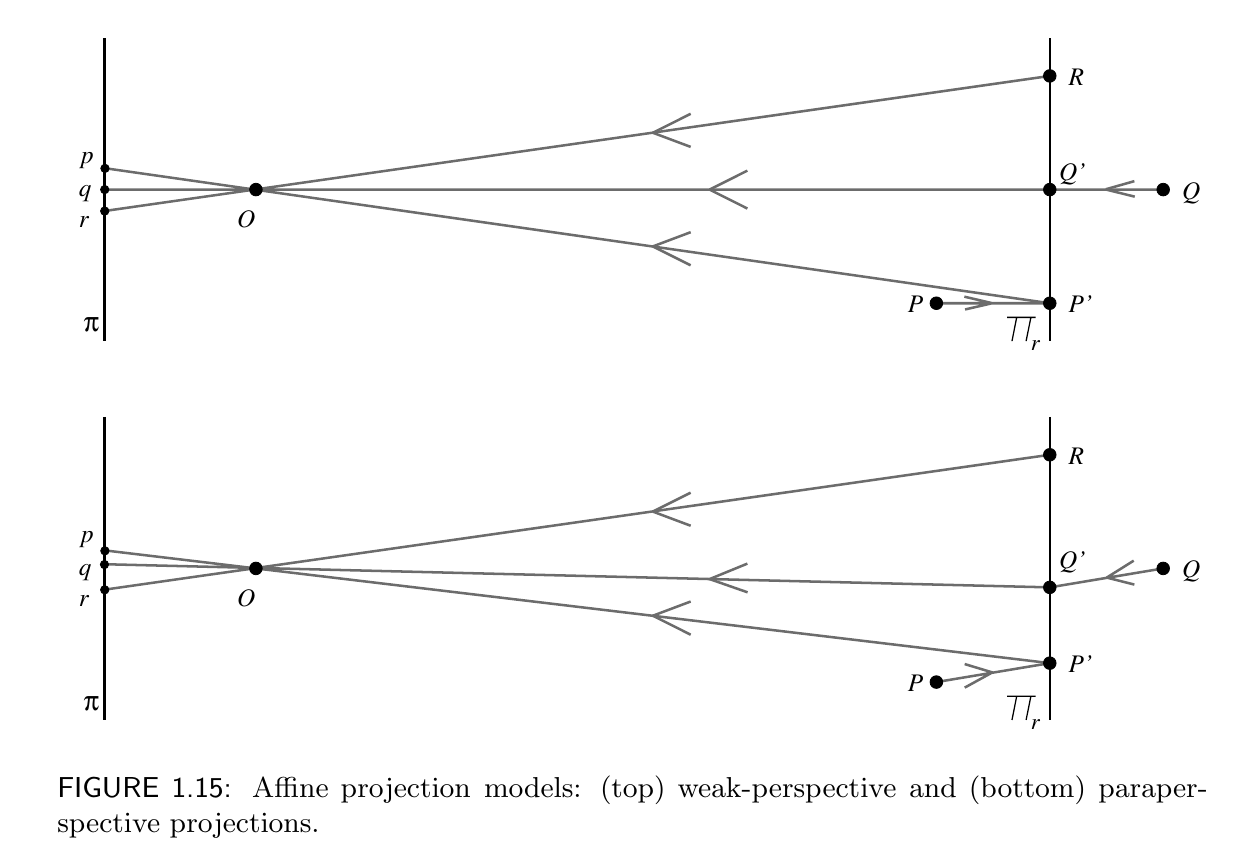
\includegraphics{img/affine_projection_models.png}}
\end{frame}}{\begin{frame}
  \frametitle{弱透视投影模型}
  \begin{eqnarray*}
    \tmmathbf{p} & = & \mathcal{M}\tmmathbf{P}
  \end{eqnarray*}
  \begin{eqnarray*}
    \tmmathbf{p} & = & \left(\begin{array}{cc}
      x & y
    \end{array}\right)^T\\
    \mathcal{M} & = & \frac{1}{Z_r} \mathcal{K} \left(\begin{array}{cccc}
      1 & 0 & 0 & 0\\
      0 & 1 & 0 & 0\\
      0 & 0 & 0 & Z_r
    \end{array}\right) \left(\begin{array}{cc}
      \mathcal{R} & \tmmathbf{t}\\
      \tmmathbf{0}^T & 1
    \end{array}\right)\\
    \tmmathbf{P} & = & \left(\begin{array}{cccc}
      X & Y & Z & 1
    \end{array}\right)^T\\
    \mathcal{K} & = & \left(\begin{array}{cc}
      \mathcal{K}_2 & p_0\\
      \tmmathbf{0}^T & 1
    \end{array}\right)\\
    \mathcal{K}_2 & = & \left(\begin{array}{cc}
      \alpha & - \alpha \cot \theta\\
      0 & \frac{\beta}{\sin \theta}
    \end{array}\right)\\
    p_0 & = & \left(\begin{array}{cc}
      x_0 & y_0
    \end{array}\right)^T
  \end{eqnarray*}
\end{frame}}{\begin{frame}
  
  \begin{eqnarray*}
    \mathcal{M} & = & \left(\begin{array}{cc}
      \mathcal{A} & \tmmathbf{b}
    \end{array}\right)\\
    & = & \frac{1}{Z_r} \mathcal{K} \left(\begin{array}{cc}
      \mathcal{R}_2 & \tmmathbf{t}_2\\
      \tmmathbf{0}^T & 1
    \end{array}\right)\\
    & = & \frac{1}{Z_r} \left(\begin{array}{cc}
      \mathcal{K}_2 & p_0\\
      \tmmathbf{0}^T & 1
    \end{array}\right) \left(\begin{array}{cc}
      \mathcal{R}_2 & \tmmathbf{t}_2\\
      \tmmathbf{0}^T & 1
    \end{array}\right)\\
    & = & \frac{1}{Z_r} \left(\begin{array}{cc}
      \mathcal{K}_2 \mathcal{R}_2 & \mathcal{K}_2 \tmmathbf{t}_2 + p_0
    \end{array}\right)\\
    & = & \frac{1}{Z_r} \left(\begin{array}{cc}
      k & s\\
      0 & 1
    \end{array}\right) \left(\begin{array}{cc}
      \mathcal{R}_2 & \tmmathbf{t}_2
    \end{array}\right)
  \end{eqnarray*}
\end{frame}}{\begin{frame}
  \frametitle{类透视投影模型}
  \begin{eqnarray*}
    \left(\begin{array}{c}
      \hat{X}\\
      \hat{Y}\\
      \hat{Z}
    \end{array}\right) & = & \left(\begin{array}{c}
      X - \frac{X_r}{Z_r} (Z - Z_r)\\
      Y - \frac{Y_r}{Z_r} (Z - Z_r)\\
      Z_r
    \end{array}\right)\\
    \mathcal{M} & = & \frac{1}{Z_r} \mathcal{K} \left(\begin{array}{cccc}
      1 & 0 & - \frac{X_r}{Z_r} & Z_r\\
      0 & 1 & - \frac{Y_r}{Z_r} & Z_r\\
      0 & 0 & 0 & Z_r
    \end{array}\right) \left(\begin{array}{cc}
      \mathcal{R} & \tmmathbf{t}\\
      \tmmathbf{0}^T & 1
    \end{array}\right)\\
    \mathcal{M} & = & \frac{1}{Z_r} \left(\begin{array}{cc}
      k & s\\
      0 & 1
    \end{array}\right) \left(\begin{array}{cc}
      \left(\begin{array}{ccc}
        1 & 0 & - \frac{X_r}{Z_r}\\
        0 & 1 & - \frac{Y_r}{Z_r}
      \end{array}\right) \mathcal{R} & \tmmathbf{t}_2
    \end{array}\right)
  \end{eqnarray*}
\end{frame}}{\begin{frame}
  \frametitle{相机标定}
  
  \resizebox{1\columnwidth}{!}{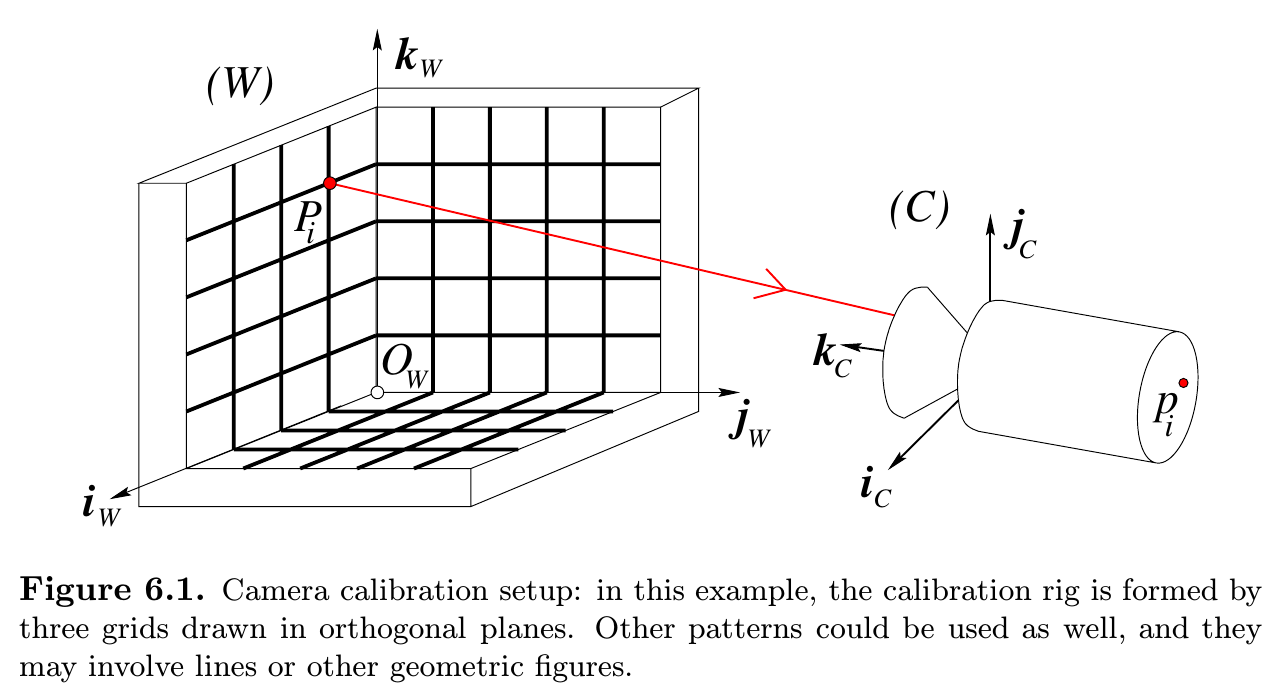
\includegraphics{img/camera_calibration_setup.png}}
\end{frame}}{\begin{frame}
  \frametitle{估计$\mathcal{M}$}
  \begin{eqnarray*}
    (\tmmathbf{m}_1 - u_i \tmmathbf{m}_3) \cdummy \tmmathbf{P}_i & = & 0\\
    (\tmmathbf{m}_{12} - u_v \tmmathbf{m}_3) \cdummy \tmmathbf{P}_i & = & 0\\
    \mathcal{P}\tmmathbf{m} & = & 0
  \end{eqnarray*}
  where
  \begin{eqnarray*}
    \mathcal{P} & = & \left(\begin{array}{ccc}
      \tmmathbf{P}_1^T & \tmmathbf{0}^T & - u_1 \tmmathbf{P}_1^T\\
      \tmmathbf{0}^T & \tmmathbf{P}_1^T & - v_1 \tmmathbf{P}_1^T\\
      \cdots & \cdots & \cdots\\
      \tmmathbf{P}_n^T & \tmmathbf{0}^T & - u_n \tmmathbf{P}_n^T\\
      \tmmathbf{0}^T & \tmmathbf{P}_n^T & - v_n \tmmathbf{P}_n^T
    \end{array}\right)\\
    \tmmathbf{m} & = & \left(\begin{array}{c}
      \tmmathbf{m}_1\\
      \tmmathbf{m}_2\\
      \tmmathbf{m}_3
    \end{array}\right)
  \end{eqnarray*}
\end{frame}}{\begin{frame}
  \frametitle{估计内参数}
  \begin{eqnarray*}
    \rho \left(\begin{array}{cc}
      \mathcal{A} & \tmmathbf{b}
    \end{array}\right) & = & \mathcal{K} \left(\begin{array}{cc}
      \mathcal{R} & \tmmathbf{t}
    \end{array}\right)\\
    \rho \left(\begin{array}{c}
      \tmmathbf{a}^T_1\\
      \tmmathbf{a}_2^T\\
      \tmmathbf{a}_3^T
    \end{array}\right) & = & \left(\begin{array}{c}
      \alpha \tmmathbf{r}_1^T - \alpha \cot \theta \tmmathbf{r}^T_2 + u_0
      \tmmathbf{r}_3^T\\
      \frac{\beta}{\sin \theta} \tmmathbf{r}_2^T + v_0 \tmmathbf{r}_3^T\\
      \tmmathbf{r}_3^{^T}
    \end{array}\right)
  \end{eqnarray*}
  $\left(\begin{array}{ccc}
    \tmmathbf{r}_1 & \tmmathbf{r}_2 & \tmmathbf{r}_3
  \end{array}\right)$为单位正交阵:
  \begin{eqnarray*}
    \rho \tmmathbf{a}_3 & = & \tmmathbf{r}_3\\
    \rho & = & \frac{\varepsilon}{| \tmmathbf{a}_3 |}\\
    \rho^2 (\tmmathbf{a}_1 \cdummy \tmmathbf{a}_3) & = & u_0\\
    \rho^2 (\tmmathbf{a}_2 \cdummy \tmmathbf{a}_3) & = & v_0
  \end{eqnarray*}
  
\end{frame}}{\begin{frame}
  \
  
  利用叉乘:
  \begin{eqnarray*}
    \rho^2 (\tmmathbf{a}_1 \times \tmmathbf{a}_3) & = & - \alpha
    \tmmathbf{r}_2 - \alpha \cot \theta \tmmathbf{r}_1\\
    \rho^2 | \tmmathbf{a}_1 \times \tmmathbf{a}_3 | & = & \frac{a}{\sin
    \theta}\\
    \rho^2 (\tmmathbf{a}_2 \times \tmmathbf{a}_3) & = & \frac{\beta}{\sin
    \theta} \tmmathbf{r}_1\\
    \rho^2 | \tmmathbf{a}_2 \times \tmmathbf{a}_3 | & = & \frac{\beta}{\sin
    \theta}
  \end{eqnarray*}
  得:
  \begin{eqnarray*}
    \cos \theta & = & - \cfrac{(\tmmathbf{a}_1 \times \tmmathbf{a}_3)
    (\tmmathbf{a}_2 \times \tmmathbf{a}_3)}{| \tmmathbf{a}_1 \times
    \tmmathbf{a}_3 | | \tmmathbf{a}_2 \times \tmmathbf{a}_3 |}\\
    \alpha & = & \rho^2 | \tmmathbf{a}_1 \times \tmmathbf{a}_3 | \sin \theta\\
    \beta & = & \rho^2 | \tmmathbf{a}_2 \times \tmmathbf{a}_3 | \sin \theta
  \end{eqnarray*}
\end{frame}}{\begin{frame}
  \frametitle{估计外参数}
  
  
  \begin{eqnarray*}
    \tmmathbf{r}_1 & = & \frac{\rho^2 \sin \theta}{\beta} (\tmmathbf{a}_2
    \times \tmmathbf{a}_3)\\
    & = & \frac{1}{| \tmmathbf{a}_2 \times \tmmathbf{a}_3 |} (\tmmathbf{a}_2
    \times \tmmathbf{a}_3)\\
    \tmmathbf{r}_2 & = & \tmmathbf{r}_3 \times \tmmathbf{r}_1
  \end{eqnarray*}
  
  \begin{eqnarray*}
    \mathcal{K}\tmmathbf{t} & = & \rho \tmmathbf{b}\\
    \tmmathbf{t} & = & \rho \mathcal{K}^{- 1} \tmmathbf{b}
  \end{eqnarray*}
\end{frame}}{\begin{frame}
  \frametitle{退化位形}
  
  $\mathcal{P}$的零空间
  \begin{eqnarray*}
    \tmmathbf{0} & = & \mathcal{P}\tmmathbf{l}\\
    & = & \left(\begin{array}{ccc}
      \tmmathbf{P}_1^T & \tmmathbf{0}^T & - u_1 \tmmathbf{P}_1^T\\
      \tmmathbf{0}^T & \tmmathbf{P}_1^T & - v_1 \tmmathbf{P}_1^T\\
      \cdots & \cdots & \cdots\\
      \tmmathbf{P}_n^T & \tmmathbf{0}^T & - u_n \tmmathbf{P}_n^T\\
      \tmmathbf{0}^T & \tmmathbf{P}_n^T & - v_n \tmmathbf{P}_n^T
    \end{array}\right) \left(\begin{array}{c}
      \tmmathbf{\lambda}\\
      \tmmathbf{\mu}\\
      \tmmathbf{\nu}
    \end{array}\right)\\
    & = & \left(\begin{array}{c}
      \tmmathbf{P}_1^T \tmmathbf{\lambda}- u_1 \tmmathbf{P}_1^T
      \tmmathbf{\nu}\\
      \tmmathbf{P}_1^T \tmmathbf{\mu}- v_1 \tmmathbf{P}_1^T \tmmathbf{\nu}\\
      \cdots\\
      \tmmathbf{P}_n^T \tmmathbf{\lambda}- u_n \tmmathbf{P}_n^T
      \tmmathbf{\nu}\\
      \tmmathbf{P}_n^T \tmmathbf{\mu}- v_n \tmmathbf{P}_n^T \tmmathbf{\nu}
    \end{array}\right)
  \end{eqnarray*}
\end{frame}}{\begin{frame}
  
  \begin{eqnarray*}
    \tmmathbf{P}^T_i \tmmathbf{\lambda}- \frac{\tmmathbf{m}_1^T
    \tmmathbf{P}_i}{\tmmathbf{m}^T_3 \tmmathbf{P}_i} \tmmathbf{P}^T_i
    \tmmathbf{\nu} & = & 0\\
    \tmmathbf{P}^T_i \tmmathbf{\mu}- \frac{\tmmathbf{m}_2^T
    \tmmathbf{P}_i}{\tmmathbf{m}^T_3 \tmmathbf{P}_i} \tmmathbf{P}^T_i
    \tmmathbf{\nu} & = & 0
  \end{eqnarray*}
  得
  \begin{eqnarray*}
    \tmmathbf{P}^T_i (\tmmathbf{m}_3 \tmmathbf{\lambda}^T -\tmmathbf{m}_1
    \tmmathbf{\nu}^T) \tmmathbf{P}_i & = & 0\\
    \tmmathbf{P}^T_i (\tmmathbf{m}_3 \tmmathbf{\mu}^T -\tmmathbf{m}_2
    \tmmathbf{\nu}^T) \tmmathbf{P}_i & = & 0
  \end{eqnarray*}
  若存在平面$\Pi$使$\Pi \cdummy \tmmathbf{P}_i = 0$,则
  \[ \left(\begin{array}{ccc}
       \Pi & 0 & 0
     \end{array}\right), \left(\begin{array}{ccc}
       0 & \Pi & 0
     \end{array}\right), \left(\begin{array}{ccc}
       0 & 0 & \Pi
     \end{array}\right), \tmmathbf{m} \]
  张成$\mathcal{P}$的零空间。
\end{frame}}{\begin{frame}
  \frametitle{考虑径向畸变}
  
  
  \begin{eqnarray*}
    \tmmathbf{p} & = & \frac{1}{z} \left(\begin{array}{ccc}
      \frac{1}{\lambda} & 0 & 0\\
      0 & \frac{1}{\lambda} & 0\\
      0 & 0 & 1
    \end{array}\right) \mathcal{M}\tmmathbf{P}\\
    \lambda & = & 1 + \sum_{p = 1}^q \kappa_p d^{2 p} \hspace{4em} q \leqslant
    3
  \end{eqnarray*}
\end{frame}}{\begin{frame}
  \frametitle{$d^2 = \hat{u}^2 + \hat{v}^2$}
  \begin{eqnarray*}
    \left(\begin{array}{c}
      \hat{u}\\
      \hat{v}
    \end{array}\right) & = & \mathcal{K}^{- 1} \left(\begin{array}{c}
      u\\
      v\\
      1
    \end{array}\right)\\
    & = & \left(\begin{array}{c}
      u \alpha^{- 1} + v \beta^{- 1} \cos \theta\\
      v \beta^{- 1} \sin \theta\\
      1
    \end{array}\right) \hspace{4em} (u_0 = v_0 = 0)\\
    \mathcal{K}^{- 1} & = & \left(\begin{array}{ccc}
      \alpha^{- 1} & \frac{\cos \theta}{\beta} & - \frac{u_0}{\alpha} -
      \frac{v_0 \cos \theta}{\beta}\\
      0 & \frac{\sin \theta}{\beta} & - \frac{u_0 \beta}{\sin \theta}\\
      0 & 0 & 1
    \end{array}\right)\\
    d^2 & = & \hat{u}^2 + \hat{v}^2\\
    & = & u^2 \alpha^{- 2} + v^2 \beta^{- 2} + 2 u \nospace v \alpha^{- 1}
    \beta^{- 1} \cos \theta
  \end{eqnarray*}
\end{frame}}{\begin{frame}
  \frametitle{估计投影矩阵}
  \begin{eqnarray*}
    \lambda \left(\begin{array}{c}
      u\\
      v
    \end{array}\right) & = & \left(\begin{array}{c}
      \frac{\tmmathbf{m}_1 \cdummy \tmmathbf{P}}{\tmmathbf{m}_3 \cdummy
      \tmmathbf{P}}\\
      \frac{\tmmathbf{m}_2 \cdummy \tmmathbf{P}}{\tmmathbf{m}_3 \cdummy
      \tmmathbf{P}}
    \end{array}\right)\\
    v (\tmmathbf{m}_1 \cdummy \tmmathbf{P}) & = & u (\tmmathbf{m}_2 \cdummy
    \tmmathbf{P})
  \end{eqnarray*}
  得
  \begin{eqnarray*}
    \mathcal{Q}\tmmathbf{n} & = & 0\\
    \mathcal{Q} & = & \left(\begin{array}{cc}
      v_1 \tmmathbf{P}^T_1 & - u_1 \tmmathbf{P}_1^T\\
      \cdots & \cdots\\
      v_n \tmmathbf{P}_n^T & - u_n \tmmathbf{P}_n^T
    \end{array}\right)\\
    \tmmathbf{n} & = & \left(\begin{array}{c}
      \tmmathbf{m}_1\\
      \tmmathbf{m}_2
    \end{array}\right)
  \end{eqnarray*}
  
\end{frame}}{\begin{frame}
  \frametitle{内参数}
  \begin{eqnarray*}
    \rho \left(\begin{array}{c}
      \tmmathbf{a}_1^T\\
      \tmmathbf{a}_2^T
    \end{array}\right) & = & \left(\begin{array}{c}
      \alpha \tmmathbf{r}_1^T - \alpha \cot \theta \tmmathbf{r}_2^T\\
      \frac{\beta}{\sin \theta} \tmmathbf{r}_2^T
    \end{array}\right)\\
    | \rho \tmmathbf{a}_1 | & = & \frac{\alpha}{\sin \theta}\\
    | \rho \tmmathbf{a}_2 | & = & \frac{\beta}{\sin \theta}\\
    \rho \tmmathbf{a}_1 \cdummy \rho \tmmathbf{a}_2 & = & - \frac{\alpha \beta
    \cos \theta}{\sin^2 \theta}\\
    \cos \theta & = & - \frac{\tmmathbf{a}_1 \cdummy \tmmathbf{a}_2}{|
    \tmmathbf{a}_1 | \cdummy | \tmmathbf{a}_2 |}\\
    \alpha & = & | \rho \tmmathbf{a}_1 | \sin \theta\\
    \beta & = & | \rho \tmmathbf{a}_2 | \sin \theta
  \end{eqnarray*}
\end{frame}}{\begin{frame}
  \frametitle{外参数$R$}
  
  
  \begin{eqnarray*}
    \tmmathbf{r}_1 & = & \frac{\varepsilon}{\sin \theta} \left(
    \frac{\tmmathbf{a}_1}{| \tmmathbf{a}_1 |} + \frac{\tmmathbf{a}_2}{|
    \tmmathbf{a}_2 |} \cos \theta \right)\\
    \tmmathbf{r}_2 & = & \frac{\varepsilon \tmmathbf{a}_2}{| \tmmathbf{a}_2 |}
  \end{eqnarray*}
  
\end{frame}}{\begin{frame}
  \frametitle{外参数$\tmmathbf{t}$}
  \begin{eqnarray*}
    \left(\begin{array}{c}
      \alpha t_x - \alpha t_y \cot \theta\\
      \cfrac{\beta t_y}{\sin \theta}
    \end{array}\right) & = & \rho \left(\begin{array}{c}
      b_1\\
      b_2
    \end{array}\right)\\
    \mathcal{M} & = & \left(\begin{array}{cc}
      \mathcal{A} & \tmmathbf{b}
    \end{array}\right)\\
    \tmmathbf{b} & = & \left(\begin{array}{ccc}
      b_1 & b_2 & b_3
    \end{array}\right)^T\\
    t_x & = & \frac{\varepsilon}{\sin \theta} \left( \frac{b_1}{|
    \tmmathbf{a}_1 |} + \frac{b_2 \cos \theta}{| \tmmathbf{a}_2 |} \right)\\
    t_y & = & \frac{\varepsilon b_2}{| \tmmathbf{a}_2 |}
  \end{eqnarray*}
  \begin{eqnarray*}
    (\tmmathbf{m}_1 - \lambda u\tmmathbf{m}_3) \cdummy \tmmathbf{P} & = & 0\\
    (\tmmathbf{m}_2 - \lambda v\tmmathbf{m}_3) \cdummy \tmmathbf{P} & = & 0\\
    \tmmathbf{m}_3 & = & \left(\begin{array}{c}
      \tmmathbf{r}_3\\
      t_z
    \end{array}\right)
  \end{eqnarray*}
\end{frame}}{\begin{frame}
  \frametitle{径向畸变}
  \begin{eqnarray*}
    d^2 & = & | (u \alpha^{- 1} + v \beta^{- 1} \cos \theta) \tmmathbf{r}_2 -
    v \beta^{- 1} \sin \theta \tmmathbf{r}_1 |^2\\
    & = & (\alpha^{- 1} \beta^{- 1} \sin \theta)^2 \left| \left( \frac{u
    \beta}{\sin \theta} + v \alpha \cot \theta \right) \tmmathbf{r}_2 - v
    \alpha \tmmathbf{r}_1 \right|^2\\
    & = & \frac{1}{| \rho \tmmathbf{a}_1 \times \rho \tmmathbf{a}_2 |^2}
    \left| \frac{u \beta}{\sin \theta} \tmmathbf{r}_2 - v (\alpha
    \tmmathbf{r}_1 - \alpha \cot \theta \tmmathbf{r}_2) \right|^2\\
    & = & \frac{| u \rho \tmmathbf{a}_2 - v \rho \tmmathbf{a}_1 |^2}{| \rho
    \tmmathbf{a}_1 \times \rho \tmmathbf{a}_2 |^2}\\
    & = & \frac{| u\tmmathbf{a}_2 - v\tmmathbf{a}_1 |^2}{| \tmmathbf{a}_1
    \times \tmmathbf{a}_2 |^2}
  \end{eqnarray*}
  
\end{frame}}}

\end{document}
